\documentclass[11pt]{article}

\usepackage{parskip}
\usepackage[colorlinks=true]{hyperref}
\usepackage{microtype}
\usepackage[margin=1.5cm]{geometry}
\usepackage{float}
\usepackage{helvet}
\renewcommand{\familydefault}{\sfdefault}
\usepackage{graphicx}
\usepackage{caption}
\usepackage{subcaption}
\usepackage[title]{appendix}
\usepackage{url}

\title{CS3210 Lab 4}
\author{Leow Li Yong \\ A0233404U}

\begin{document}

\section{Testing and Results}
Each configuration was run 5 times.
For each run, the computation and communication times for each worker was recorded.
The results obtained are shown below:
\begin{figure}[H]
  \centering
  \begin{subfigure}[t]{0.45\textwidth}
    \centering
    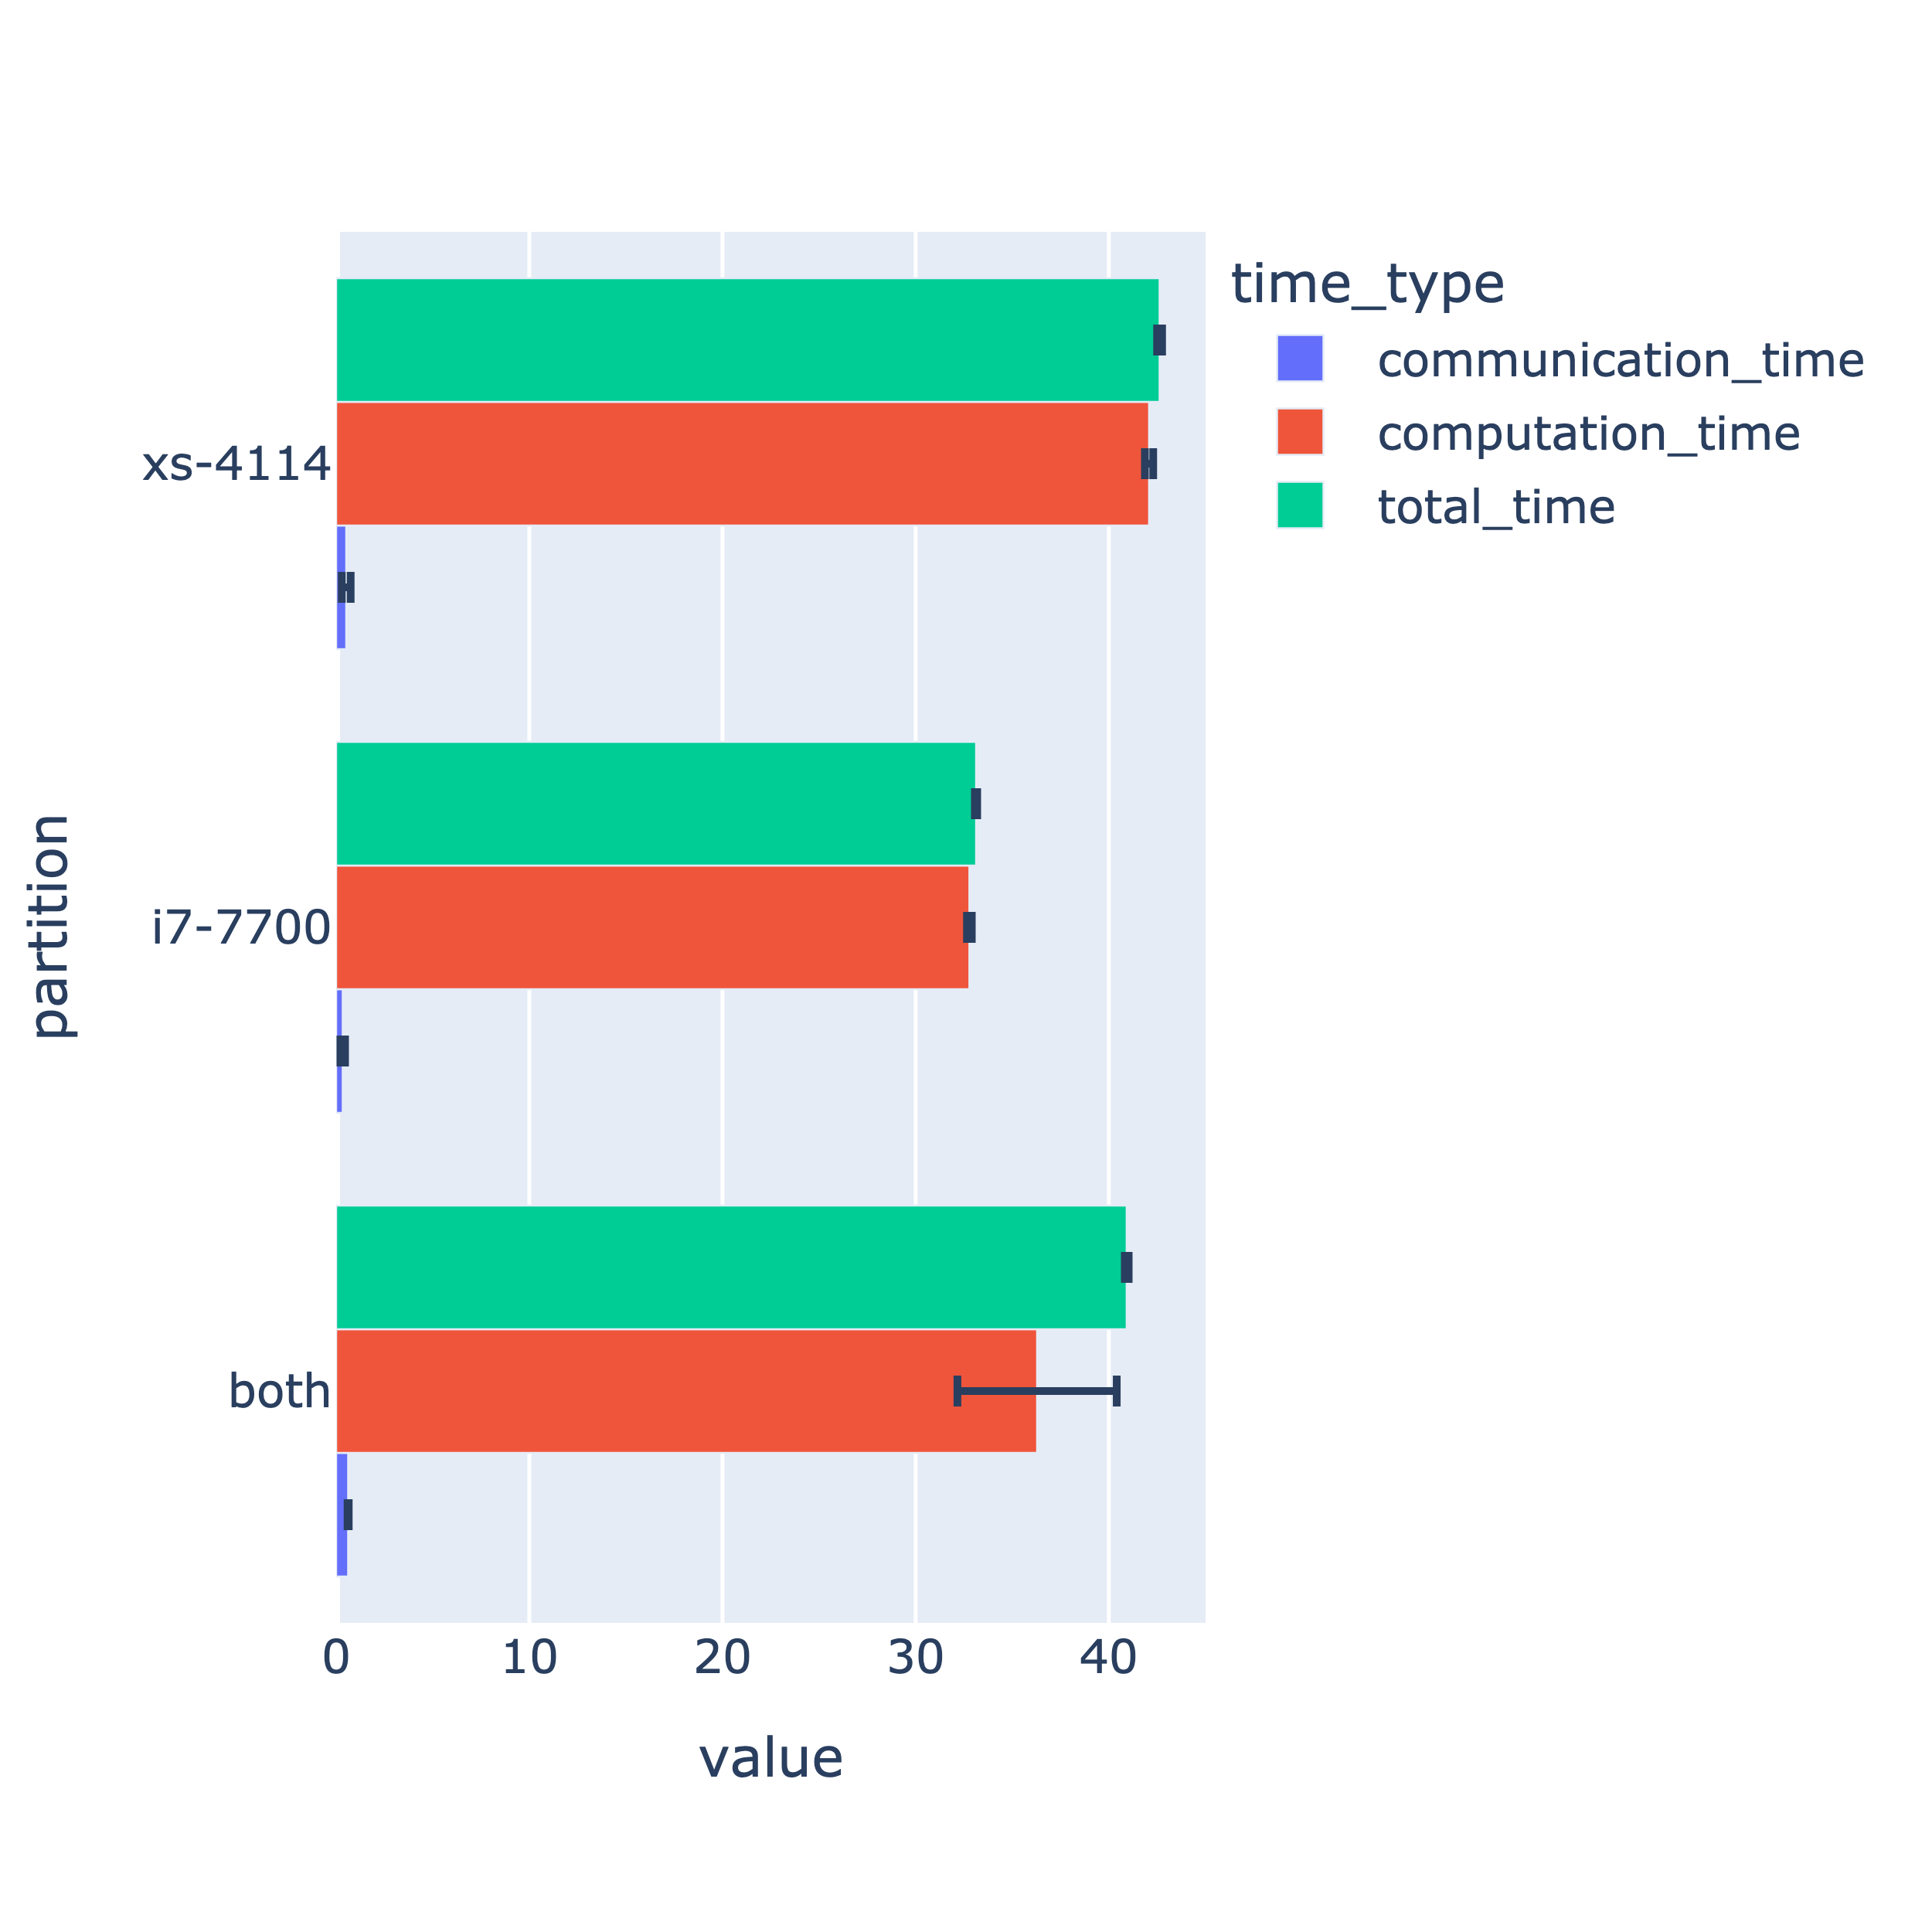
\includegraphics[width=\textwidth]{figures/main-1.png}
    \caption{Exercise 10, performance vs node type}
    \label{fig:main-1}
  \end{subfigure}
  \begin{subfigure}[t]{0.45\textwidth}
    \centering
    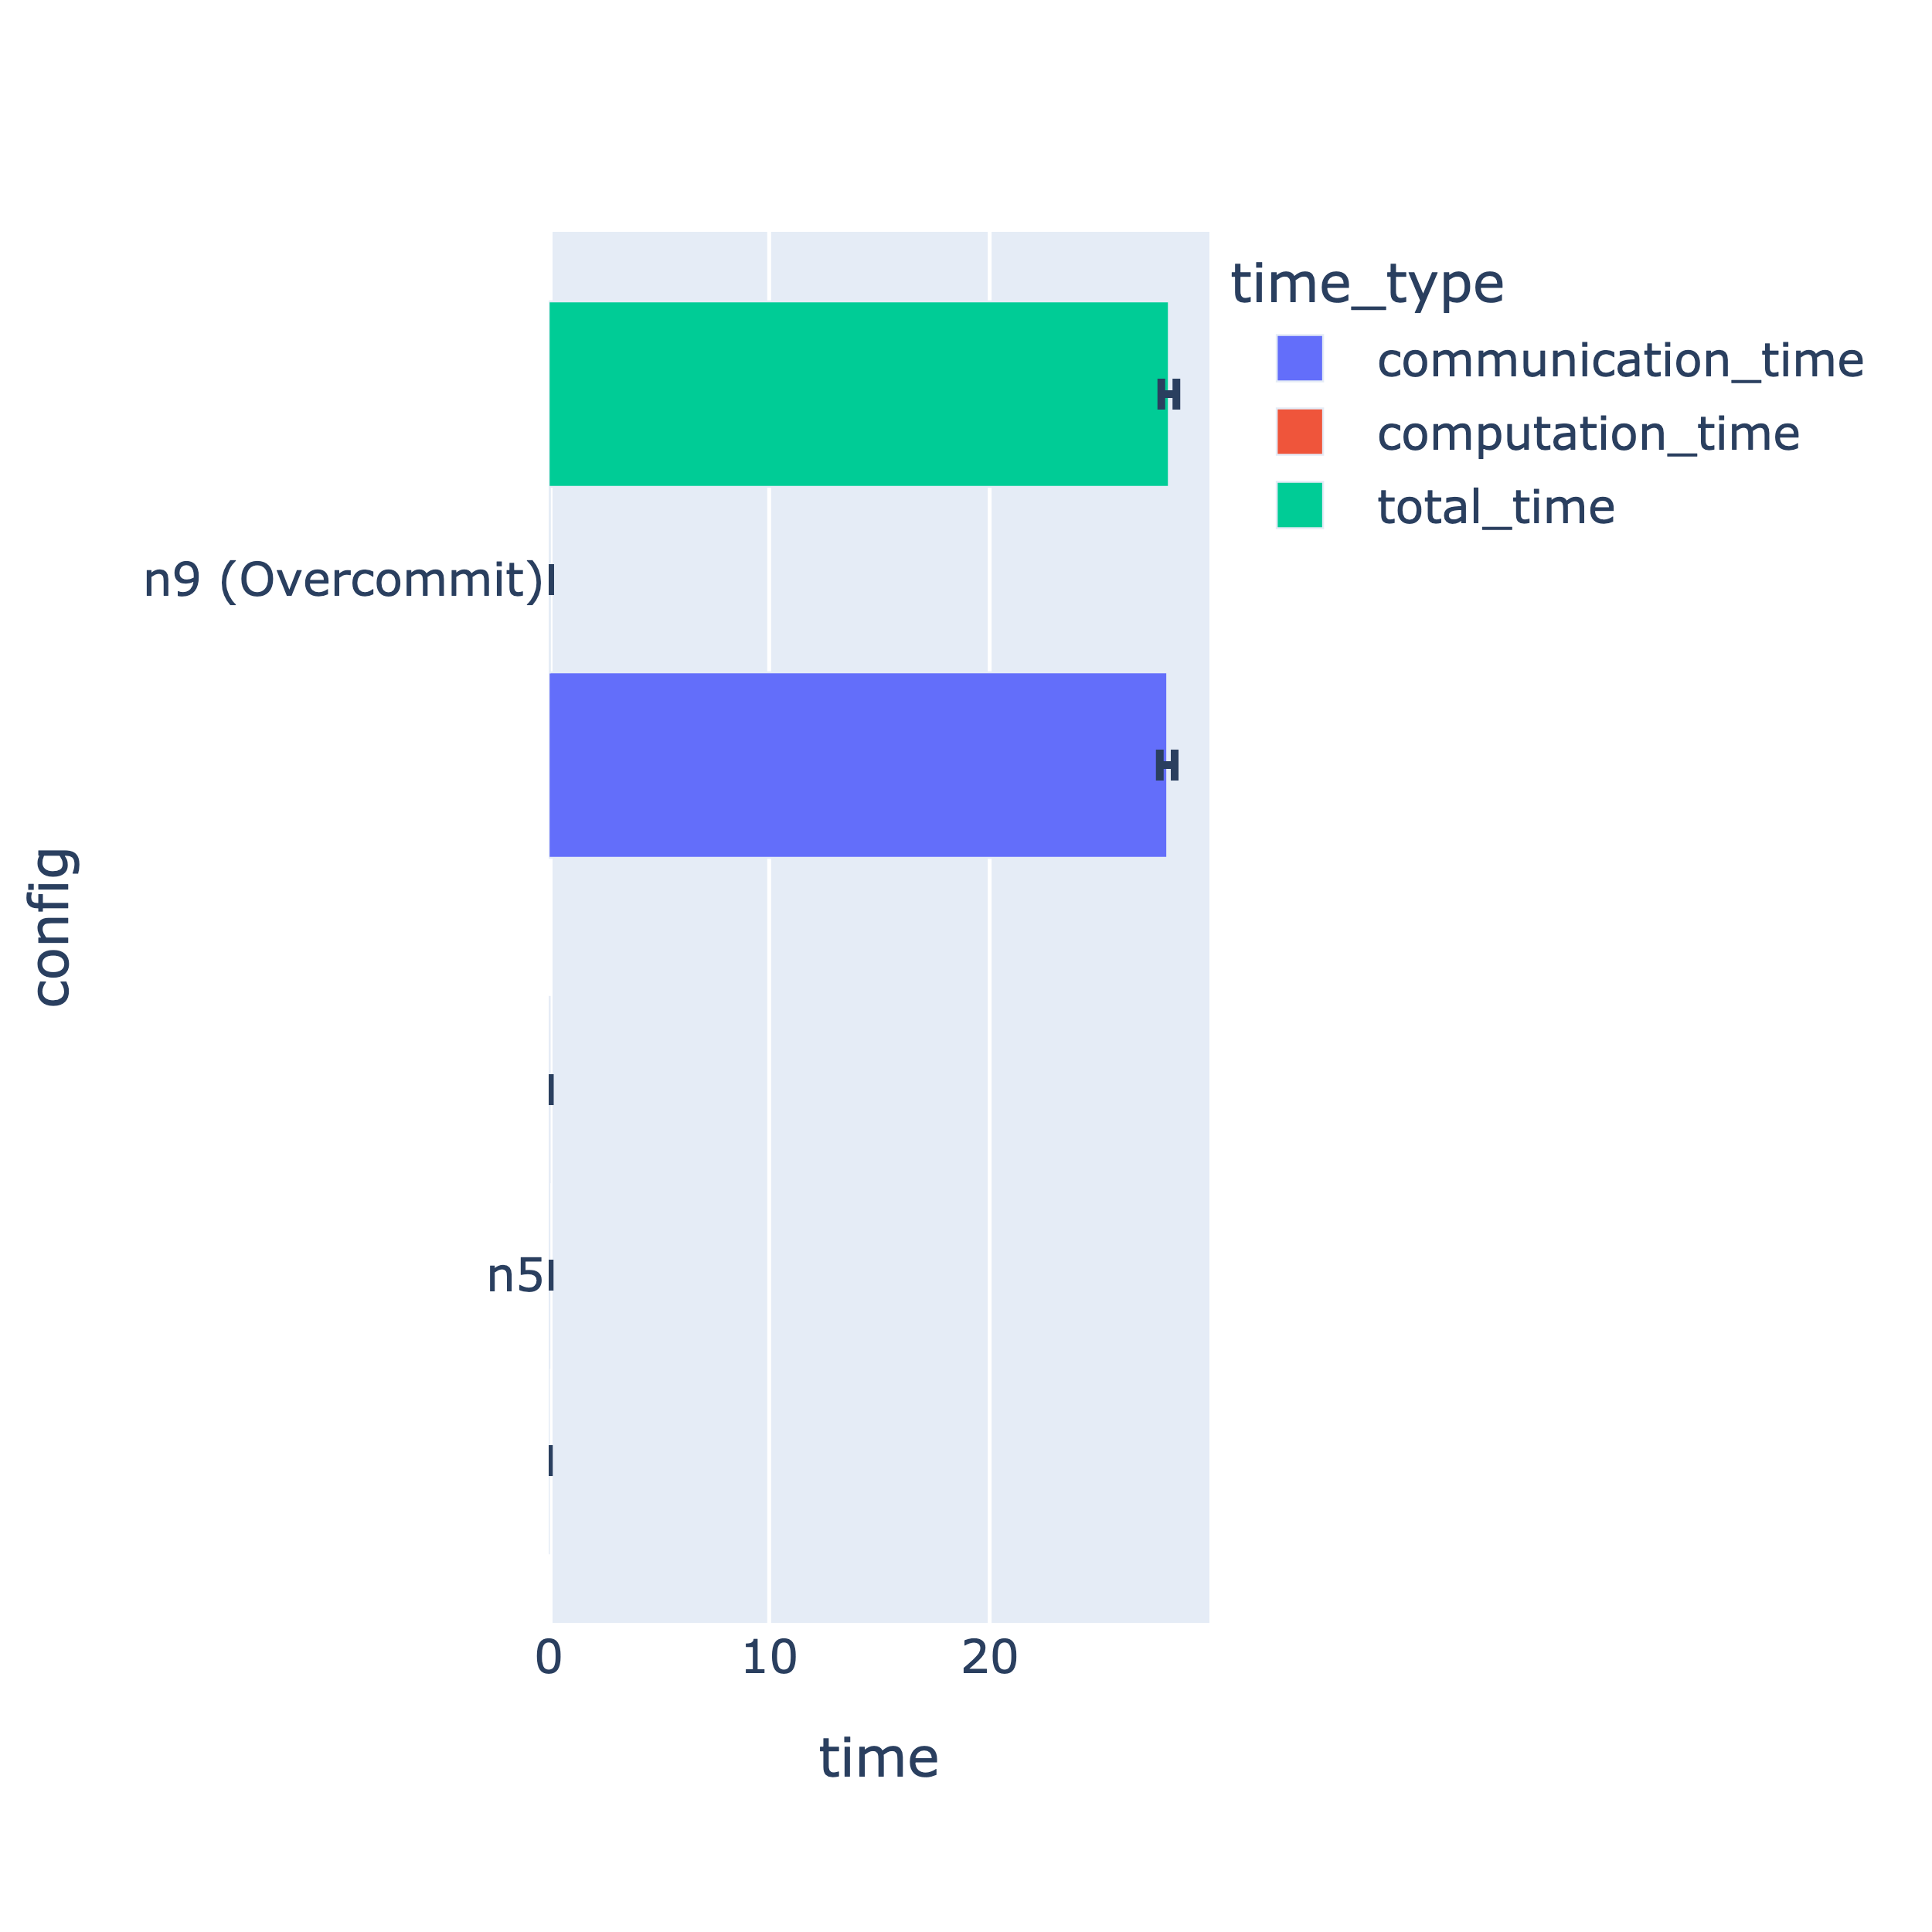
\includegraphics[width=\textwidth]{figures/main-2.png}
    \caption{Exercise 11, performance vs i7-7700 node configuration}
    \label{fig:main-2}
  \end{subfigure}
  \caption{Performance Results, averaged across workers and repetitions, with standard deviation error bars}
\end{figure}

\section{Exercise 10 - Comparing Different Nodes}
From \ref{fig:main-1},
running all processes on a single i7-7700 node achieves the best performance,
followed by a cyclic distribution on one i7-7700 node and 1 xs-4114 node,
and running all processes on a xs-4114 node achieves the worst performance.

Performance is mostly bottle necked by computation time.
The difference between the i7-7700 and xs-4114 node is due to clock speed,
and the configuration that uses 2 nodes is bottle necked by the slower xs-4114 node
as shown by the larger standard deviation in computation time between workers.

\section{Exercise 11 - 5 nodes vs 9 nodes (Overcommitted)}

From figure \ref{fig:main-2},
the configuration with 9 nodes (overcommitted) achieves significantly worse performance than the configuration with 5 nodes.
The main cause of this is the high communication time that is bottle necking the 9 node configuration.

The master process sequentially sends the matrices' data row by row to each worker node using a blocking send.
In the 9 node configuration, there is more than 1 process per logical CPU core on the i7-7700 (8 logical cores).
The large number of blocking sends and receives would lead to numerous context switches, leading to longer communication times.

To improve the performance of the overcommitting implementation, the code can be modified to use asynchronous communication.
Every row and element of the required matrices' can be sent/received asynchronously before waiting for the operation to complete.
This should reduce the number of context switches and communication time.

The tests were repeated with asynchronous message passing and the following results were obtained:

\begin{figure}[H]
  \begin{center}
    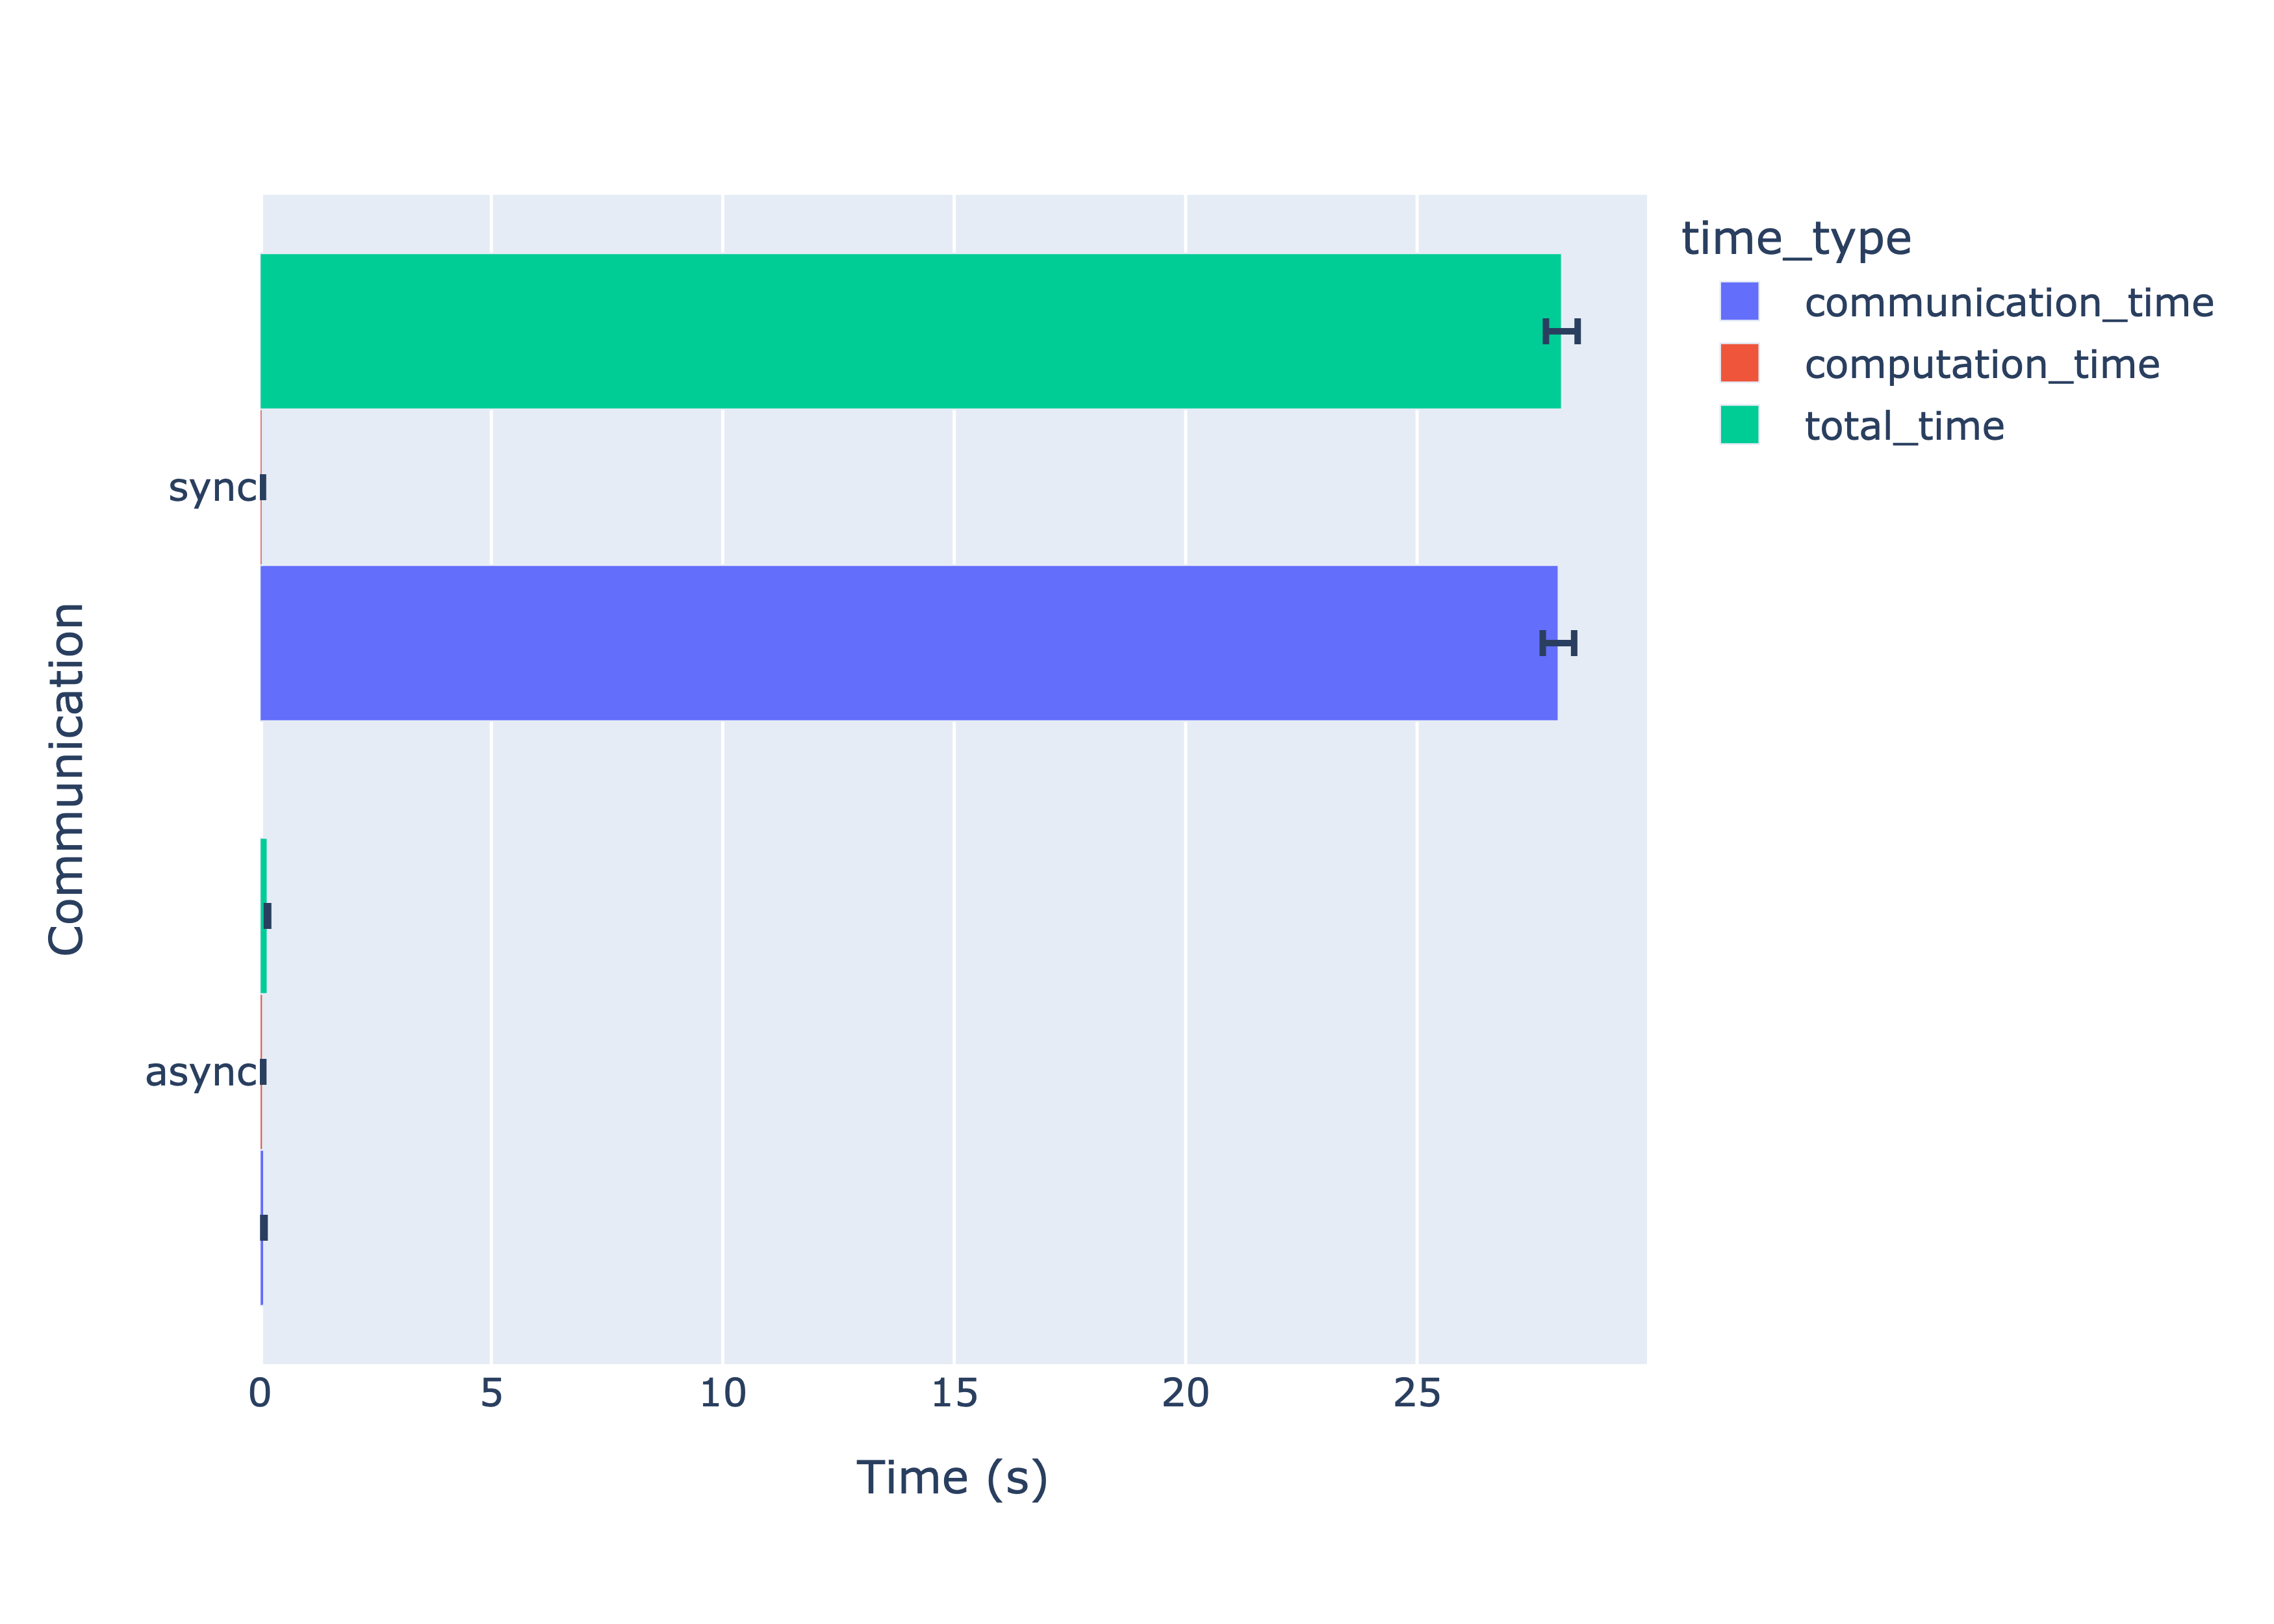
\includegraphics[width=0.8\textwidth]{figures/async.png}
  \end{center}
  \caption{Bar plots comparing performance between async and sync communication for 9 node (overcommit) config}\label{fig:async}
\end{figure}

From figure \ref{fig:async},
there is a significant improvement in communication time, leading to the same relative reduction in total time.

\clearpage
\begin{appendices}
  All files referenced can be found in \url{https://github.com/ginloy/CS3210-Labs/tree/main/L4}.
  \section{Reproduction}

  \begin{itemize}
    \item \href{https://github.com/ginloy/CS3210-Labs/blob/main/L4/test.sh}{\path{test.sh}} was used to run the slurm commands and parse results into a csv.

    \item Raw data can be found in \href{https://github.com/ginloy/CS3210-Labs/blob/main/L4/results2.csv}{\path{results2.csv}} and
      \href{https://github.com/ginloy/CS3210-Labs/blob/main/L4/results-async.csv}{\path{results-async.csv}}
      
    \item \href{https://github.com/ginloy/CS3210-Labs/blob/main/L4/graphs.ipynb}{\path{graphs.ipynb}} was used to process the data and generate all graphs.
  \end{itemize}

  \section{Code changes for Exercise 12}
  \href{https://github.com/ginloy/CS3210-Labs/blob/main/L4/ex12.patch}{\path{ex12.patch}}  

\end{appendices}

\end{document}
